\section{Exercise 4}
\subsection*{4.1}
\begin{figure}[H]
	\centering
	\begin{subfigure}[b]{0.45\textwidth}
		\centering
		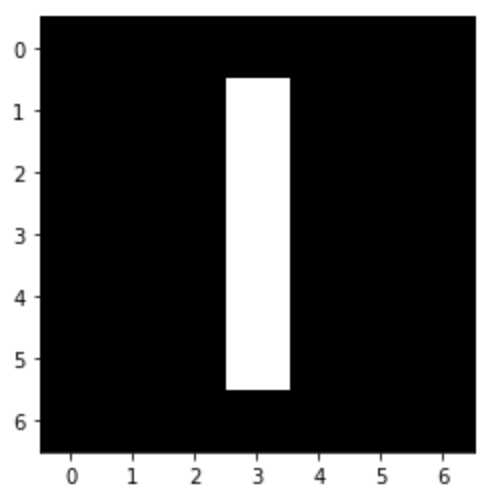
\includegraphics[width=\textwidth]{Materials/digit}
		\caption{The chosen digit / input image.}
	\end{subfigure}
	\hfill
	\begin{subfigure}[b]{0.45\textwidth}
		\centering
		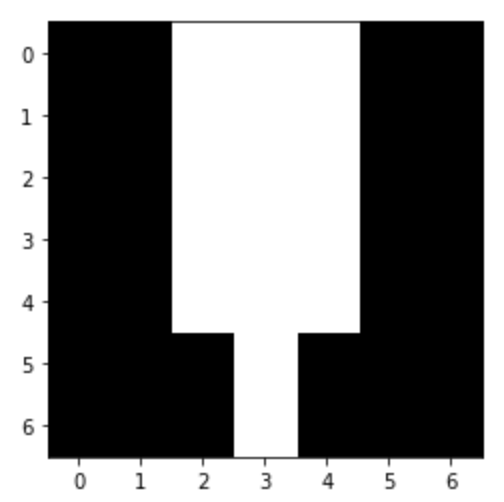
\includegraphics[width=\textwidth]{Materials/m1res}
		\caption{Dilation with mask 1.}
		\label{m1res}
	\end{subfigure}
	\hfill
	\\
	\begin{subfigure}[b]{0.45\textwidth}
		\centering
		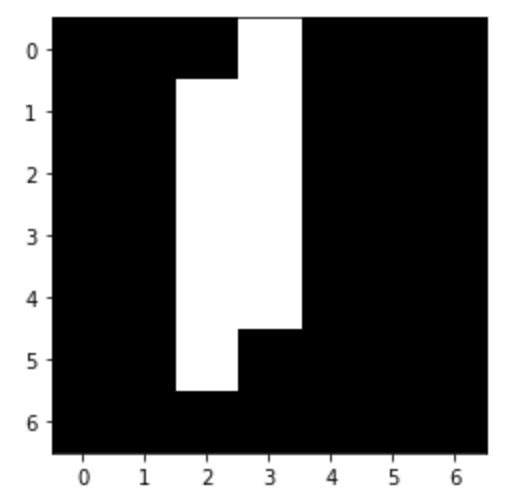
\includegraphics[width=\textwidth]{Materials/m2res}
		\caption{Dilation with mask 2.}
		\label{m2res}
	\end{subfigure}
	\hfill
	\begin{subfigure}[b]{0.45\textwidth}
		\centering
		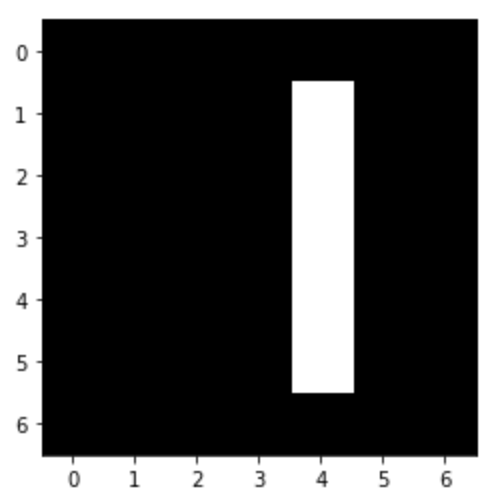
\includegraphics[width=\textwidth]{Materials/m3res}
		\caption{Dilation with mask 3.}
		\label{m3res}
	\end{subfigure}
	\caption{Results of dilation with masks from the exercise.}
\end{figure}
\textbf{i.:}The structuring element does not need to be symmetric. As can be seen in \autoref{m1res} the resulting image after dilation adds the 'T' shape to the input image. The centre pixel is defined as the middle one in the 3 by 3 grid, i.e. the white pixel in the second row.\\
\textbf{ii.:} The structuring element does not need to have an odd number of pixels in both directions. In \autoref{m2res} we see the diagonal pattern added to the input image. The centre pixel is the lower right black pixel.\\
\textbf{iii.:} The structuring element does not need to have the middle pixel set to true. As seen in \autoref{m3res} the output simply gets shifted. The centre pixel is the middle black pixel.\\
The code for this exercise can be seen in \autoref{e41code}.
\begin{figure}[H]
	\centering
	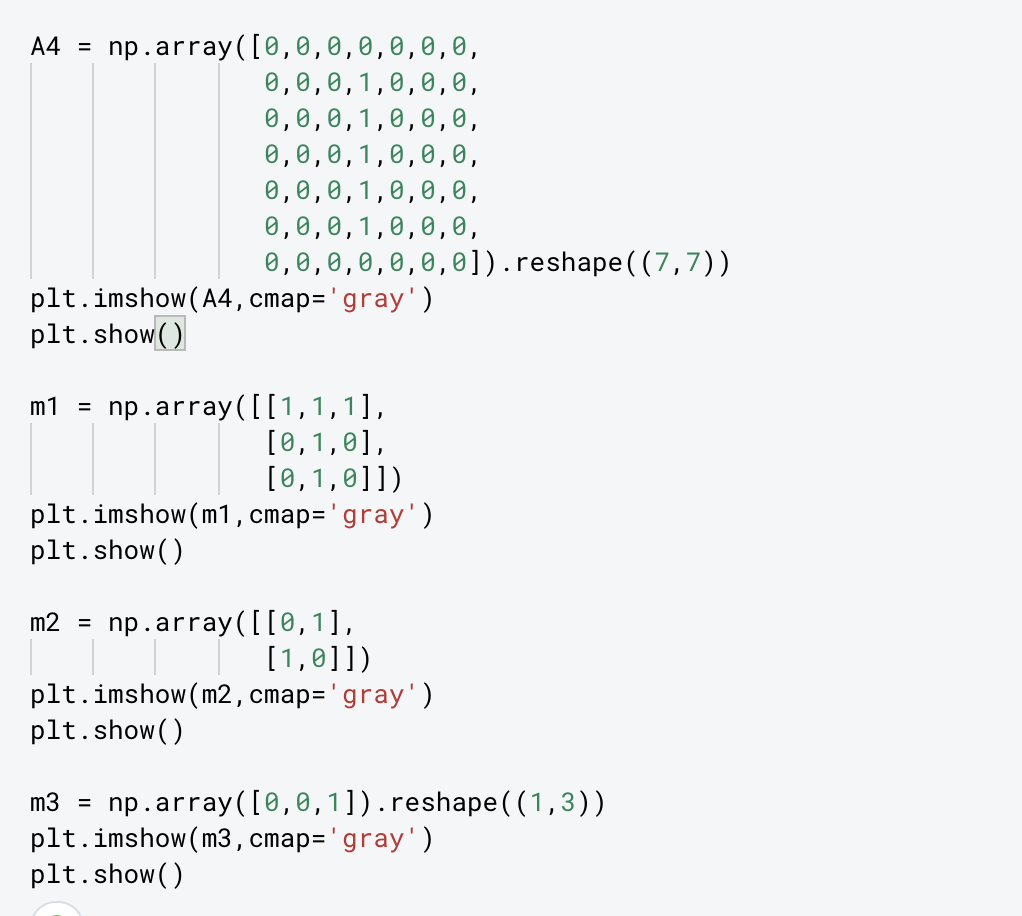
\includegraphics[width=0.7\linewidth]{Materials/e41code}
	\caption{Code for exercise 4.1.}
	\label{e41code}
\end{figure}

\subsection*{4.2}
\begin{figure}[H]
	\centering
	\begin{subfigure}[b]{0.45\textwidth}
		\centering
		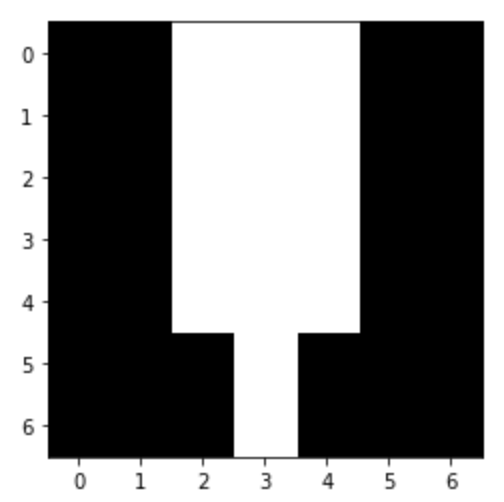
\includegraphics[width=\textwidth]{Materials/m1res}
		\caption{Mask 1.}
	\end{subfigure}
	\hfill
	\begin{subfigure}[b]{0.45\textwidth}
		\centering
		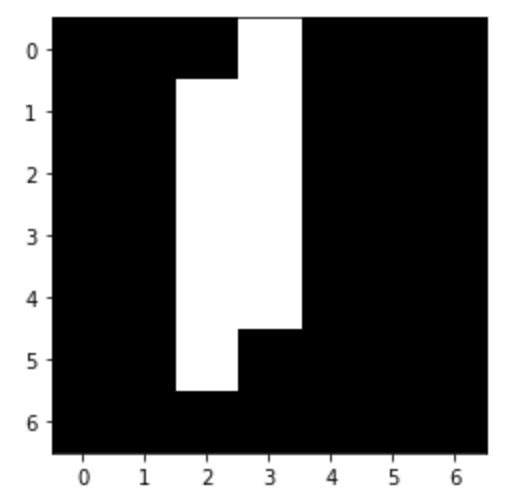
\includegraphics[width=\textwidth]{Materials/m2res}
		\caption{Mask 2.}
	\end{subfigure}
	\hfill
	\\
	\begin{subfigure}[b]{0.45\textwidth}
		\centering
		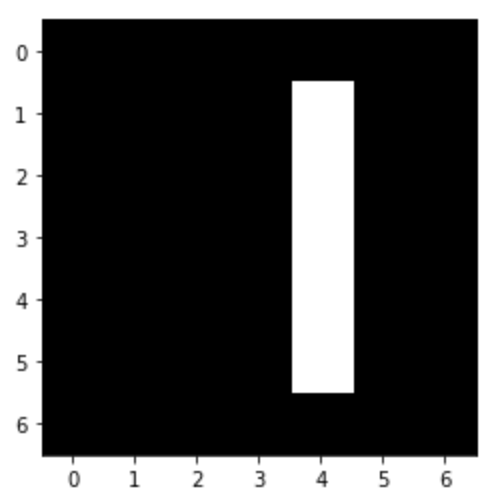
\includegraphics[width=\textwidth]{Materials/m3res}
		\caption{Mask 3.}
	\end{subfigure}
	\caption{Results of dilation of masks with input image.}
	\label{dilation}
\end{figure}
When performing the dilation with the input image on the masks we get the exact same results as before due to the commutative property of dilation. This indeed means we can interchange the input image and mask and get the same results. This can be useful if either the mask or the input image contains \textit{many} more 'true' pixels than the other, then interchanging the mask and the input image such that we only need to perform dilation on a few 'true' pixels might speed things up.\\
The results of this exercise can be seen in \autoref{dilation} and the code for this exercise can be seen in \autoref{e42code}.
\begin{figure}[H]
	\centering
	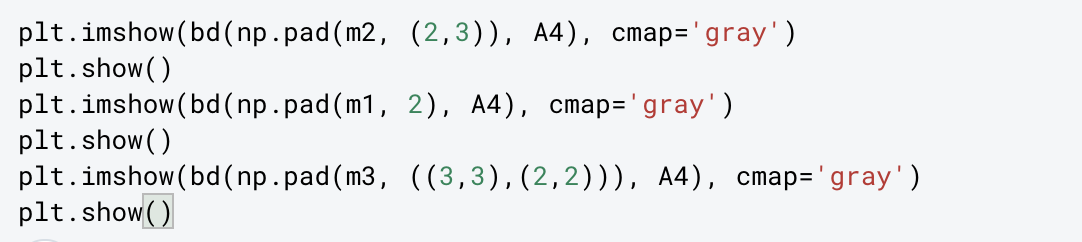
\includegraphics[width=0.7\linewidth]{Materials/e42code}
	\caption{Code for exercise 4.2.}
	\label{e42code}
\end{figure}